\section{Feature Demonstration}

\subsection{Images}

I made a couple of latex commands that make inserting images a bit shorter. I made a command called \code{\insertimage{}{}{}}, which takes three arguments: the image filename, the caption, and the label. I also made a command called \code{\insertbigimage{}{}{}}, which does the same thing, but for big images that are too wide to be placed in a single column. \Cref{normal_image,big_image} are the result of using these commands (Though the big image is too big to fit on this page).

\insertimage{photos/c3.png}{Example Image}{normal_image}

\insertbigimage{photos/R6.pdf}{Example Big Image (Made using MATLAB)}{big_image}

\subsection{Math}

This isn't really a feature of my template, but more a feature of \LaTeX \ itself. 
Here is some Math:
\begin{equation}
    C = A \times B = \begin{bmatrix}
        c_{11} & c_{12} & c_{13} \\
        c_{21} & c_{22} & c_{23} \\
        c_{31} & c_{32} & c_{33}
    \end{bmatrix}
\end{equation}
Here is some more ChatGPT gave me:
\begin{align*}
    F(s) &= \mathcal{L} \{ f(t) \} \\
    &= \int_{0}^{\infty} f(t) e^{-st} \, dt
\end{align*}

I made a couple of commands that make writing math a bit easier. For example, I made a command called \code{\E{}}, which takes one argument, the exponent. For example, \code{\E{3}} will display as $\E{3}$. I also made a command called \code{\abs{}}, which takes one argument, the value to be enclosed in absolute value bars. For example, \code{\abs{-3}} will display as $\abs{-3}$ \footnote[1]{Only works in a math environment, either in an align/equation environment or between \$ \$ symbols. By the way footnotes are also a thing in \LaTeX.}


\subsection{Tables}

I don't have any custom commands to make tables, but I can still make them My recommendation is to use ChatGPT to generate the table for you.
\begin{table}[h!]
    \centering
    \begin{tabular}{ll}
        \toprule
        \textbf{Column 1} & \textbf{Column 2} \\
        \midrule
        Data 1 & Data 2 \\
        More Data 1 & More Data 2 \\
        Even More Data 1 & Even More Data 2 \\
        Dummy Data 1 & Dummy Data 2 \\
        Another Data 1 & Another Data 2 \\
        \bottomrule
    \end{tabular}
    \caption{A small table}
    \label{table_dummy}
\end{table}

I (mostly ChatGPT) have configured a way for latex to read \code{.xlsx} and \code{.csv} files, which can be seen in \cref{table_csv}. This table was generated using a \code{.csv} file, with the column names changed to have nice math in them. \Cref{table_csv} shows this.

\begin{table}[h]
    \centering
    \begin{tabular}{ccccc} % Adjust the widths as needed
        \toprule
        \begin{tabular}[c]{@{}c@{}}Reco-\\rding\end{tabular} & 
        \begin{tabular}[c]{@{}c@{}}$\Delta P_{\text{avg}}$ \\$ - \Delta P_{\text{avg}}'$ (m)\end{tabular} &
        \begin{tabular}[c]{@{}c@{}}$\Delta P_{\text{fin}}$ \\$ - \Delta P_{\text{fin}}'$ (m)\end{tabular} & 
        \begin{tabular}[c]{@{}c@{}}$\Delta P_{\text{max}}$ \\$ - \Delta P_{\text{max}}'$ (m)\end{tabular} \\
        \midrule
        \csvreader[head to column names, late after line=\\]{tables/data.csv}{}
        {\csvcoli & \csvcolii & \csvcoliii & \csvcoliv}
        \bottomrule
    \end{tabular}
    \caption{Data from \code{tables/data.csv}}
    \label{table_csv}
\end{table}

\newpage

\subsection{Code}

I also made a command for inline code, \code{\code{}}. This command takes one argument, the code to be displayed. For example, \code{\code{print("Hello World")}} will display as \code{print("Hello World")}. Groundbreaking, I know. 

I also made a command for code blocks, \code{\codeblock{}{}} \codeblock{python}{Example Python Code}{code_example}{code/python.py}
This command takes four arguments: the language, the caption, the label, and the filename. Mostly, I'd reccommend using \code{\onecolumn} before using this command. This way, the code won't do any weird overflowing stuff, like you can see on line 24 in \cref{code_example}.


\subsection{Tikz Plots and Pictures}

If you want a really simple figure, it may be worth it to use Tikz which is an inbuilt \LaTeX \  figure rendering tool.
Here are a couple of examples of things you can do. For most things it's more worth it to either hand draw it or use draw.io. Either way \crefrange{tikz1}{tikz4} show some examples of what you can do with Tikz.

\begin{figure}[h]
    \centering
    \begin{tikzpicture}[scale=1.25, >=Latex]
        % Define rotation angles
        \def\angleKminusOne{45}
        \def\angleK{20}
        
        % Draw axes
        \draw[thick,->] (0,0) -- (0,4) node[anchor=south] {Northings (m)};
        \draw[thick,->] (0,0) -- (4,0) node[anchor=west] {Eastings (m)};
        
        % Define coordinates for points
        \coordinate (O) at (0,0);
        \coordinate (pk-1) at (1,1);
        \coordinate (pk) at (3,2.75);
        

        %Pk-1
        %square
        \node[draw, rectangle, minimum width=1cm, minimum height=0.6cm, anchor=center, rotate=\angleKminusOne, fill=red!25, dashed] at (pk-1) {};

        %position label
        \node[anchor=north west] at (pk-1) {$(p_{x_{k-1}},p_{y_{k-1}})$};
        %velocity vector
        \draw[thick,->] (pk-1) -- ++(\angleKminusOne:1.5cm) node[anchor= west] {$v_{k-1}$};
        % angle
        \draw[thick,dashed] (pk-1) -- ++(0cm, 1.5cm); 
        \draw[->] (pk-1) +(90:0.5cm) arc (90:\angleKminusOne:0.5cm);
        \node at ($(pk-1)+(0.35cm, 0.8cm)$) {$\theta_{k-1}$};
        
        %Pk
        %square
        \node[draw,rectangle, minimum width=1cm, minimum height=0.6cm,anchor=center,rotate=\angleK, fill=red!50] at (pk) {};
        %position label
        \node[anchor=north west] at (pk) {$(p_{x_{k}},p_{y_{k}})$};
        %velocity vector
        \draw[thick,->] (pk) -- ++(\angleK:1.5cm) node[anchor= west] {$v_{k}$};
        % angle
        \draw[thick,dashed] (pk) -- ++(0cm, 1.5cm); 
        \draw[->] (pk) +(90:0.5cm) arc (90:\angleK:0.5cm);
        \node at ($(pk)+(0.35cm, 0.6cm)$) {$\theta_{k}$};
        
    \end{tikzpicture}
    \caption{Representation of State Vector Components in Physical Space}
    \label{tikz1}
\end{figure}

\begin{figure}[h]
    \centering
    \definecolor{WaterColor}{RGB}{1,176,241}
    \begin{tikzpicture}[scale=0.75, >=Latex]
        % Clipping path for the jar shape
        \begin{scope}
            \clip (0,0) -- (0,4) -- (4,4) -- (4,0) arc[start angle=360, end angle=180, x radius=2, y radius=0.5];
            % Drawing the water, now reaching the elliptical bottom
            \fill[WaterColor] (0,0) rectangle (4,2);
        \end{scope}
        
        % Drawing the grey rectangles
        \fill [WaterColor] (4,2) arc[start angle=0, end angle=360, x radius=2, y radius=0.5]; %top water ellipse
        \fill [WaterColor] (4,0) arc[start angle=0, end angle=360, x radius=2, y radius=0.5]; %bottom water ellipse
        \draw [WaterColor!60] (4,2) arc[start angle=0, end angle=180, x radius=2, y radius=0.5]; %back surface ellipse
        \draw [thick, dotted] (0,0) arc[start angle=180, end angle=0, x radius=2, y radius=0.5]; % Dotted top half of the elliptical base
        \fill[gray] (0.8,0) rectangle (1.2,4); % left electrode
        \fill [gray] (1.2,0) arc[start angle=0, end angle=360, x radius=0.2, y radius=0.05]; %left electrode base
        \fill [gray] (1.2,4) arc[start angle=0, end angle=360, x radius=0.2, y radius=0.05]; %left electrode cap
        \fill[gray] (2.8,0) rectangle (3.2,4); % right electrode 
        \fill [gray] (3.2,0) arc[start angle=0, end angle=360, x radius=0.2, y radius=0.05]; %left electrode base
        \fill [gray] (3.2,4) arc[start angle=0, end angle=360, x radius=0.2, y radius=0.05]; %left electrode cap
        \draw [WaterColor!60] (0,2) arc[start angle=180, end angle=360, x radius=2, y radius=0.5]; %front surface ellipse
        
        % Drawing multiple red arrows at different y positions with the new arrow style
        \foreach \y in {0.6, 2.2, 3.8} {
        % Drawing a wire, then a smaller capacitor, then another wire
        \draw[red] (1.2,\y) -- (1.8,\y) to[C, color=red] (2.2,\y) -- (2.8,\y);
        }
        % Drawing the jar with rounded corners and an elliptical bottom
        \draw [very thick, rounded corners] (0,4) -- (0,0);
        \draw [very thick] (4,0) -- (4,4);
        % Measure labels for water and air sections
        \draw[<->,thick] (4.5,0) -- (4.5,2) node[midway,fill=white,anchor=west]{$xH$};
        \draw[<->,thick] (4.5,2) -- (4.5,4) node[midway,fill=white,anchor=west]{$(1-x)H$};

        % Adding nodes for air and water
        \node at (-0.5, 3) {$\varepsilon_a$}; % Node A in the middle of the air
        \node at (-0.5, 1) {$\varepsilon_w$}; % Node B in the middle of the water
        \draw [very thick] (0,0) arc[start angle=180, end angle=360, x radius=2, y radius=0.5]; % Elliptical base

    \end{tikzpicture}
    \caption{Ideal model of Capacitive Sensor}
    \label{tikz2}
\end{figure}

\begin{figure}[h]
    \centering
    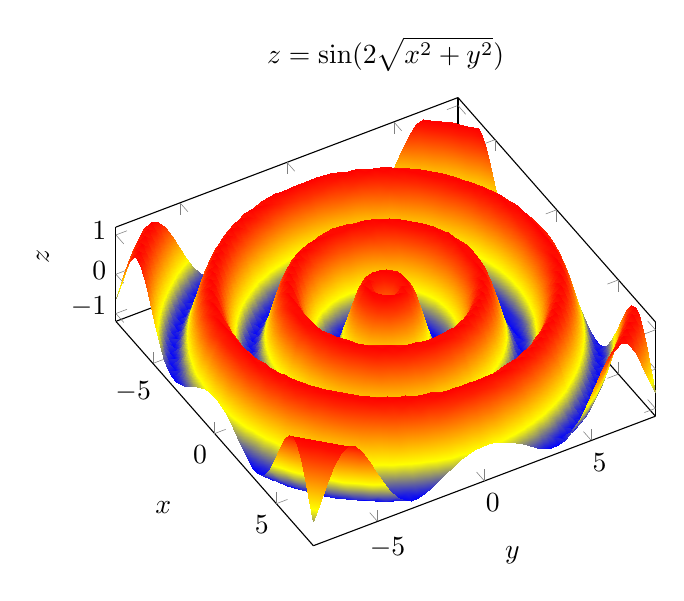
\begin{tikzpicture}
    \begin{axis}[
        title={$z = \sin(2\sqrt{x^2 + y^2})$},
        xlabel={$x$},
        ylabel={$y$},
        zlabel={$z$},
        domain=-8:8,
        y domain=-8:8,
        view={60}{70},
        samples=50
    ]
    \addplot3[
        surf,
        shader=interp,
    ]
    {sin(deg(2*sqrt(x^2 + y^2)))};
    \end{axis}
    \end{tikzpicture}
    \caption{3D plot of $z = \sin(2\sqrt{x^2 + y^2})$}
    \label{tikz3}
\end{figure}


\begin{figure}[h]
    \centering
    \begin{circuitikz}[american voltages]
        \draw
          (0,0) to [short, *-] (6,0)
          to [V, l_=$\mathrm{j}{\omega}_m \underline{\psi}^s_R$] (6,2) 
          to [R, l_=$R_R$] (6,4) 
          to [short, i_=$\underline{i}^s_R$] (5,4) 
          (0,0) to [open, v^>=$\underline{u}^s_s$] (0,4) 
          to [short, *- ,i=$\underline{i}^s_s$] (1,4) 
          to [R, l=$R_s$] (3,4)
          to [L, l=$L_{\sigma}$] (5,4) 
          to [short, i_=$\underline{i}^s_M$] (5,3) 
          to [L, l_=$L_M$] (5,0); 
        \end{circuitikz}
    
    % Caption and label for the figure
    \caption{Random Circuit I found on the internet lol} 
    \label{tikz4}
\end{figure}

circuits in particular are a major pain. If you want a circuit in your document, make it in Microcap and screenshot that (like \cref{normal_image})


\subsection{tcolorboxes}
\begin{tcolorbox}[colback=red!5!white,colframe=red!50!black,title=My nice heading]
    This is a tcolorbox with a heading. I never use tcolourboxes except for the inline code command. They're just small tcolourboxes. I thought I'd put it here anyway in case people want to use them.
\end{tcolorbox}

\begin{tcolorbox}[colback=green!5!white,colframe=green!75!black]
    Upper part of my box.
    \tcblower
    Lower part of my box. WOW!
\end{tcolorbox}


\subsection{refreencing}

You can also reference stuff. If you're doing lab reports youd be surprised how little you reference - though this does depend on the subject. If you dont want references just delete the \code{.bib} file and remove the lines in the \code{main.tex} file that have stuff to do with bibliography. That should be it I think.

Here is an example of an IEEE style reference using \code{cite()}: \cite{normal_distribution_wiki_page}


